\documentclass[]{article}
\usepackage[a4paper, margin=2.5cm]{geometry}
\usepackage{fancyhdr, graphicx, lastpage}
\usepackage{titlesec}
\usepackage{amsmath}
\usepackage{caption}
\usepackage{graphicx}
\usepackage{float}
\usepackage{matlab-prettifier}
\usepackage[sorting=none, backend=biber, style=ieee]{biblatex} 
\addbibresource{Thesis.bib}
\setcounter{secnumdepth}{4}
\makeatletter
\def\input@path{"./MATLAB Software"}
\makeatother
\graphicspath{{./figures/}}
\graphicspath{{./images/}}
\allowdisplaybreaks
\usepackage[parfill]{parskip} % Change indents to line breaks between paragraphs
\emergencystretch=1em % Used to make badness error for bibliography go away

\title{Data Analysis for Predictive Maintenance of a Straightening Machine in the Steel Industry}
\date{September 2023}
\author{Paul Barron}

\begin{document}
\pagenumbering{roman}
\maketitle
\newpage

\section*{Acknowledgments}
I would like to thank my supervisors Daniel Rönnow and Oscar Bautista Gonzalez for their guidance and patience.
I would like to thank the University of Gävle for offering a Masters program available to take as distance education.
Finally I would like to thank my partner, Alex Hamelin, for her support.
\newpage

\section*{Abstract}
% Some general comment on the reasons for the project
The availability of industrial machinery  is crucial to any business operating in the manufacturing sector. Mechanical failures halt production and unplanned downtime is disruptive and costly. Small failures can lead to catastrophic failures which exponentially increases downtime and repair costs. Identifying a degradation condition before reaching catastrophic failure is key to increasing and maintaining machine availability. On the other hand, one does not want to waste resources performing maintenance where it is not required. For these reasons a large field of academic work is dedicated to analyzing the health of a machine, predicting it's remaining life and thus preventing these kind of failures.

% What the project is about
This thesis analyses a tube straightening machine used in the steel industry with the end goal of implementing a condition monitoring strategy. The data for this project comes from a real world application from a multinational manufacturer of steel products. It was obtained using the existing sensors and data acquisition system. The project serves as a study of the existing infrastructure (available sensors) and it's suitability for implementing a condition monitoring strategy. The work is the first step in a larger study and does not attempt to perform any implementation or fault identification.

% Outling of project steps
The data consists of an hour per day taken from a two week duration. It is prepossessed to isolate periods where the machine is operating and separated into cycles. Each of these pulses is then further processed to extract time and frequency domain features. The features of each signal are compared with each other using the $R^{2}$ coefficient of determination to find signals that are correlated and a semi manual method is used to select a combination of features. The same process is performed between signals for each feature. 

% The conclusions of the project
A number of linear regression models are created based on the results from the correlated features as well as some multivariate models. These are then compared using a FIT metric. Potential clustering of machine states are highlighted based on observations in the feature combinations. The conclusions drawn from this study include identification of relationships between signals, potential non-linear correlations and suggestions for future data collection going forward.
\clearpage

\tableofcontents
\newpage
\listoffigures
\listoftables
\newpage

\fancypagestyle{plain}{
	\fancyhf{}
	\fancyhead[C]{Data Analysis for Predictive Maintenance of a Straightening Machine in the Steel Industry}
	\cfoot{\thepage} 
}
\pagestyle{plain}

\pagenumbering{arabic}
\section{Introduction}
\subsection{Background}
% What is condition monitoring
Condition monitoring (CM) is the process of predicting machine health through a combination of sensor data and software algorithms. Sensors measure parameters like vibration, temperature and acoustic emissions that provide input data to an algorithm which outputs health metrics. This allows operators to gain some understanding of when a machine might fail and perform some preventative intervention. The ability to monitor equipment health and predict remaining lifetime has valuable benefits. Avoiding unplanned downtime and catastrophic failure allows the extraction of more value from existing resources.

% Discuss why CM is important
The application of CM and predictive maintenance is a large area of research in the machine and manufacturing industry. Of course it is not only limited to machines being utilized on other engineering structures like bridges and also biological systems. 
% Discuss more specifically bearing vibration analysis
A common application of condition monitoring is the vibration analysis of rotating machines. The degradation of a bearing results changes in the vibration signal which can be a indicator of bearing health. 
%Even more specifically a tube straightening machine
One such example of an industrial machine that uses roller bearings is a rotary tube straightening machine. These are used as a finishing process in the steel industry for the manufacturing of metal tubes. They are crucial for straightening the tube in the longitudinal direction and improving ovality of the product. 

% Explain why condition monitoring would be useful for a straightening machine
Straightening machines, like many other industrial machines, are expensive to acquire and down time is costly. Performance may also be impacted by the machine being in poor condition and in need of maintenance. Thus it is in the interest of the operators to be able to schedule planned maintenance instead of having unplanned downtime and catastrophic failures.

% Challenges for CM
%Advantage of having access to this data
While there is a large array of research around bearing vibration and condition monitoring, all machines have their nuances so one CM strategy is not necessarily suitable for all. No research specifically involving CM on a straightening machine could be found. Unlike a simulation study, CM requires real-world data and it is not readily available unless working inside of a company. This study has access to real world data from such a machine and serves as a great opportunity to do an analysis.

% Big Data -> What is Feature Extraction
One of the challenges implementing CM is that there are often huge amounts of data to process and sift through. Thus Feature extraction can be used to reduce the amount of data whilst preserving the information from the raw data. By analyzing the features one can then select the most relevant channels and reduce the data even further. How to select the best features is another area of research for exists many automated and non-automated methods. This study uses a semi-automated method using the R-squared correlation coefficient to select the most appropriate features.

% Supervised vs Unsupervised learning
Another difficulty with condition monitoring research is the limited access to failure data meaning one is often forces to perform unsupervised learning
Supervised classification uses labeled data to perform the task. However, in real applications this is often not the case. More common is to have partially labeled or totally unlabeled data and thus a different set of techniques exist for unsupervised or semi-supervised learning. Here the data analysis is geared towards pattern recognition and clustering since no failure data is available to go with the data.

\subsection{Project Aim}
The aim of this project is to examine the existing data collection strategy for a tube straightening machine and make some suggestions as to whether it is possible to perform condition monitoring and/or remaining life analysis for this machine. The first step analyze the available data that can be be attained using the existing sensors and data acquisition system. The end foal is to begin developing a strategy that will assist the company to know when the machine requires maintenance. The specific goals of this project are summarized as follows:
\begin{itemize}
\item Understand what signals are related to each other.
\item Understand the signals from a statistical point of view.
\item Identify which features are of significance and which are not useful for condition monitoring i.e. which features may represent degradation condition.
\end{itemize}
\clearpage  
\section{Theory}
\subsection{System}
Rotary straightening machines, Figures \ref{straighteningImage2}, \ref{straighteningImage3} and \ref{straighteningImage6}, are industrial machinery developed to straighten and improve ovality of a metal pipes. A tube is fed through a series of roller pairs undergoing a series of bending moments to straighten the tubes. A number of different configurations for this type of machine exist with six and 10 rolls being common. At least some of the rollers are driven by motors which grip and rotate the tube while feeding it through the machine.

"Hydraulic or mechanical systems gradually and precisely apply force to specific points on the bent tube. The machine is designed to use controlled bending and flexing forces to counteract the existing deformities in the tube. By applying force at the correct locations, the machine can induce controlled plastic deformation, gradually bringing the tube back to its intended straight form."

The rollers' profile is not the same as the tube radius but are hyperbolic/parabolic in shape and only contact the tube in 3 places. This shape allows it to accommodate different tube diameters by adjusting the gap or height between the upper and lower rollers as well as the angle between them and the tube. The rollers can be adjusted from parallel to the pipe up to approximately 45 degrees with the upper rollers being adjusted in opposite angle to lower rollers.

"While passing through the machine, the tube is subjected to two specific straightening forces: pressure straightening and bend (or offset) straightening."

Modern machines are equipped with sensors monitor the amount of force being applied, the deformation of the tube, and other relevant parameters. This feedback allows the machine to make real-time adjustments to the straightening process for optimal results. These sensors, while controlling the process itself can also be used for condition monitoring purposes.

While many papers describe theoretical analysis of the mechanical mechanisms of such machine there are none that cover condition monitoring of such machine nor provide real life data from such machine.

\begin{figure}[H]
	\centering
	\includegraphics[keepaspectratio]{straightening2.png}
	\caption{An image of the roller profile of a straightening machine~\cite{ma2020effect}}
	\label{straighteningImage2}
\end{figure}

%\begin{figure}[H]
%	\centering
%	\includegraphics[]{straightening1.jpg}
%	\caption{A straightening machine~\cite{kato2014straightening}}
%	\label{straighteningImage1}
%\end{figure}

\begin{figure}[H]
	\centering
	\includegraphics[]{straightening3.jpg}
	\caption{An image of a straightening machine layout~\cite{ma2021analysis}}
	\label{straighteningImage3}
\end{figure}

%\begin{figure}[H]
%	\centering
%	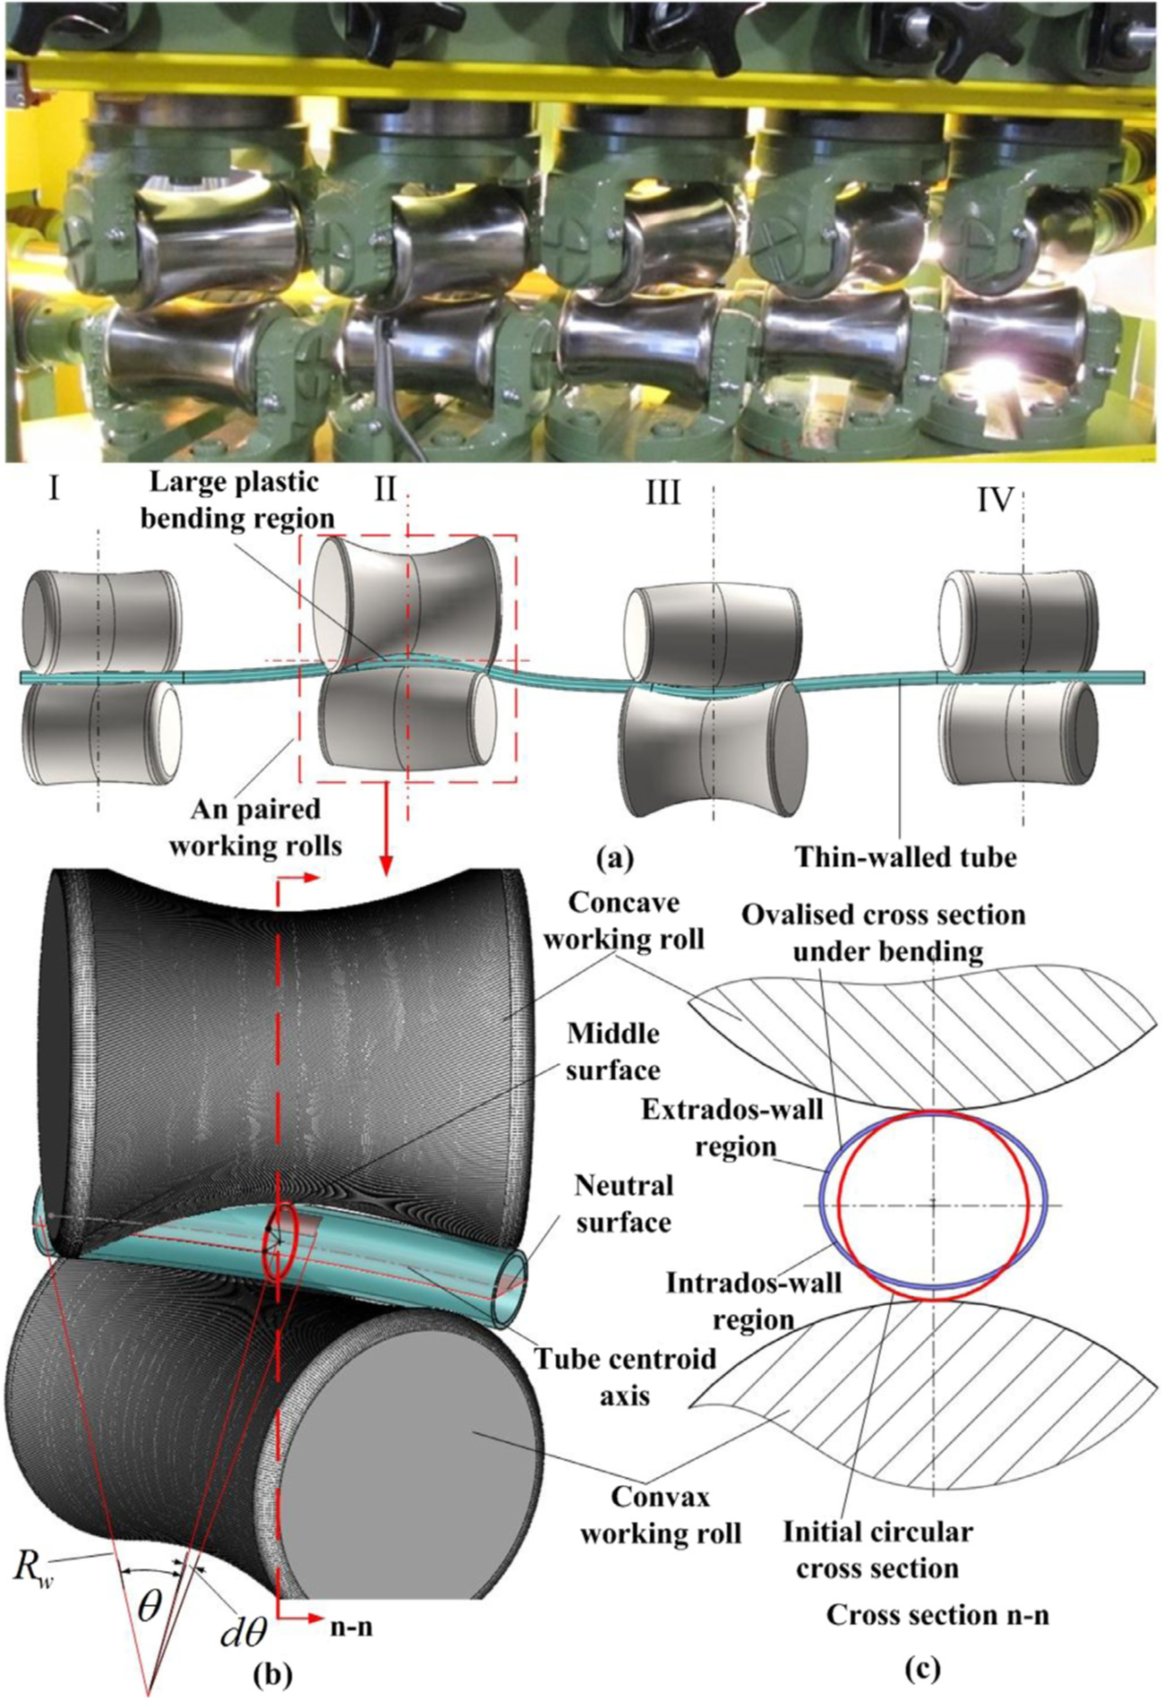
\includegraphics[width=90mm, keepaspectratio]{Straightening5.png}
%	\caption{A straightening machine~\cite{zhang2019modeling}}
%	\label{straighteningImage5}
%\end{figure}

\begin{figure}[H]
	\centering
	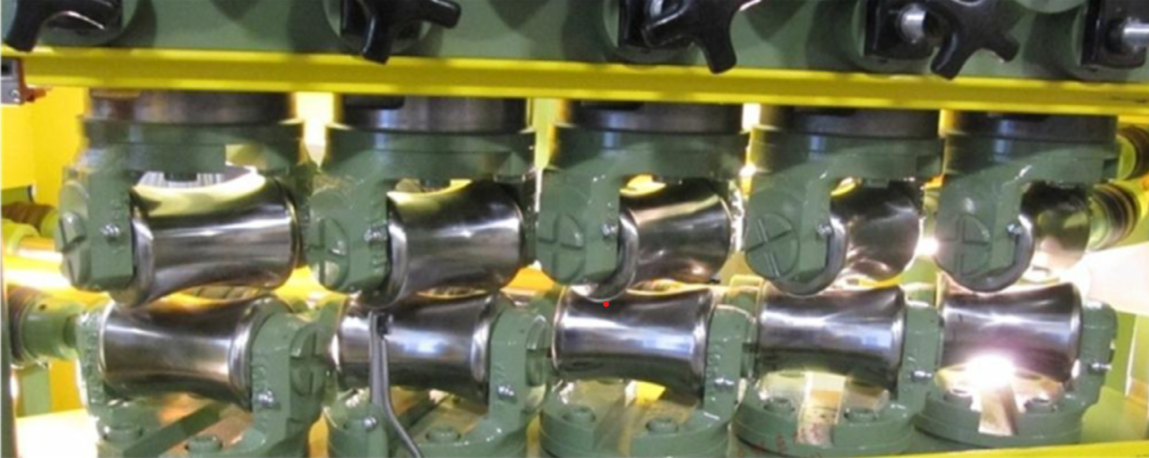
\includegraphics[width=\textwidth, keepaspectratio]{Straightening6.png}
	\caption{A 10 roller straightening machine~\cite{zhang2019modeling}}
	\label{straighteningImage6}
\end{figure}

%Condition Monitoring with Vibration Signals: Compressive Sampling and Learning Algorithms for Rotating Machines - Textbook
"Machine condition monitoring techniques can be grouped into the following: vibration monitoring, acoustic emission monitoring, a fusion of vibration and acoustic, electric motor current monitoring, oil analysis, thermography, visual inspection, performance monitoring, and trend monitoring."

~\cite{soualhi2021novel}.
[A Review on Vibration-Based Condition Monitoring of Rotating Machinery]

~\cite{yoshimura2009effect}. Significant research exists on the mechanical analysis of such machines ~\cite{kato2014straightening}~\cite{ma2020effect}~\cite{ma2021analysis}~\cite{yu2018theoretical}~\cite{das1991mechanics} however there are no studies on the monitoring of such system or non-theoretical studies using real life data.

\subsection{Feature Extraction}
%Statistical learning? 

%Why Feature Extraction?
One problem with high dimensional data is that it requires vast amounts of storage. By firstly extracting features and secondly deciding which are irrelevant one can reduce the amount of data that needs to be stored and processed while still retaining the essence of the data.

"Because slewing bearing is a large low-speed heavy-load bearing, vibration signal is insufficient. On the other hand, because of the influence of the
environment, it is difficult to obtain failure data of slewing bearing under actual working conditions, and tests also will entails high costs, so that the failure data is limit."This paper discusses a life forcasting model~\cite{wang2016multiple}

%Feature Extraction in general
Feature extraction is the process of computing numerical values from raw data in order to reduce big data sets but preserves the information. Machine learning algorithms suffer from high volumes of data and information redundancy?
"The main task of feature selection is to select a subset of features that are the most relevant to the classification problem." ~\cite{ahmed2020condition}

%Feature extraction used in condition monitoring/degradation
Feature extraction techniques for condition monitoring are used for estimating degradation trends ~\cite{caesarendra2017review} ~\cite{adams2017comparison}.

%Techniques for selecting features
This paper talks about "top sensitive features"~\cite{bleakie2013feature}.
This paper talks about defines feature goodness metrics of correlation (Corr), monotonicity (Mon) and robustness (Rob) ~\cite{zhang2016degradation}.

%Automatic feature extraction? Manual Feature extraction?
Acoustic emission signals. Ant colony optimization-based feature selection methods?~\cite{liao2010feature}.

Advanced monitoring of machining operations~\cite{teti2010advanced}


This paper discusses a life forecasting model~\cite{wang2016multiple}
This PhD thesis does this..~\cite{martin2017unsupervised}

\subsection{Time Domain Features} 	
Statistical features, Impulsive Metrics, 
\subsubsection{Cross correlation}
???
\subsubsection{Mean}
The mean is the average value of the signal.
$$ \bar{x} = \frac{\sum^N_{i=1} x_i}{N} $$
\subsubsection{Standard Deviation}  
The standard deviation is the square root of variance measures the dispersion of a data set relative to its mean. 
$$ \sigma =\frac{\sum^N_{i=1}(x_i-\bar{x})^2}{(N-1)\sigma^2} $$
\subsubsection{Root Mean Square (RMS)}
Square root of the mean squared.
$$ x_{RMS} = \sqrt{\frac{1}{N} \sum^N_{i=1}x^2_i} $$
\subsubsection{Shape Factor}
Root mean square divided by the mean of the absolute value. It is dependent on the signal shape and independent of the units
$$ x_{SF} = \frac{ x_{rms} }  {\frac{1}{N}\sum^N_{i=1}|x_i|} $$
\subsubsection{Kurtosis}
Kurtosis is a statistical measure of the tailedness of a distribution. It gives us the total degree of outliers present. An increase in the number of outliers, and thus an increase in the Kurtosis metric, can be a indication of an impending fault.
$$ x_{kurt} = \frac{\sum^N_{i=1}(x_i-m)^4)}{(N-1)\sigma^4} $$ 
\subsubsection{Skewness} 
A measure of asymmetry of through probability density function. Faults can sometimes be revealed through asymmetric distribution.
$$ x_{skew} = \frac{\sum^2_{i=1}(x_i-m)^3}{(N-1)\sigma^3} $$
\subsubsection{Peak Value}
Maximum value of a signal
$$ x_p = max(x_i) $$ 
\subsubsection{Impulse Factor} 
The maximum absolute value divided by the mean of absolute value. Comparison of the height of the peak to the average value.
$$ x_{IF} = \frac{x_p}{(\frac{1}{N}\sum^N_{i=1}|x_i|)} $$  
\subsubsection{Crest Factor} 
Divide the maximum absolute value of a signal by the RMS value.
Faults can often be detected as a peakiness of signals before they become evident in the energy (RMS).
$$ x_{crest} = \frac{x_p}{\sqrt{\frac{1}{N}}\sum^N_{i=1}x^2_i} $$
\subsubsection{Clearance Factor} 
Peak value divided by the squared mean value of the square roots of the absolute values. For a healthy bearings this feature is maximum and decreases as faults develop.
$$ x_{clear} = \frac{x_p}{(\frac{1}{N}\sum^N_{i=1}\sqrt{|x_i|})^2} $$
\subsubsection{Signal to Noise Ratio}
Ratio of signal power to noise power in decibels.
\subsubsection{Signal-to-Noise And Distortion}
Ratio of total harmonic component power to fundamental power.
\subsubsection{Total Harmonic Distortion}
Ratio of total signal power to total noise-plus-distortion power.

\subsection{Frequency Domain Features}
In order to computer the frequency features one must first compute a power spectrum.
\subsubsection{Band Power}
The band power is the area beneath the graph, within a frequency range, of the power spectral density vs the frequencies.
the power of a signal in the selected frequency range.
The area under the spectrum curve within the chosen band limits.
\subsubsection{Peak Amplitude}
Peak amplitude is the height of the maximum frequency value on the power spectrum.
\subsubsection{Peak Frequency}
Peak frequency is the value of the frequency which has the highest peak.

\subsection{Coefficient of Determination, R-squared}
Compute cross correlations between 2 features (this can maybe be a feature as well?)
Calculate R2, which relates to the variance in linear regression models.
\begin{align*}
 R^2 &= 1 - \frac{\textrm{sum squared regression (SSR)}}{\textrm{total sum of squares (SSR)}} \\ 
 &= 1 - \frac{\Sigma(y_i - \hat{y_i})^2}{\Sigma(y_i - \bar{y_i})^2} 
\end{align*}
An R-squared value of 1 means that the two signals are perfectly linear where as a value of 0 or closed to zero means there is no or next to none linear relationship.
\subsubsection{Feature Selection}
Once the features have been calculated one must discover the most useful and relevant features. 

This paper mentions feature selection techniques like ANOVA F-Test, Recursive Feature Elimination, Model Importance, Feature Correlation Clustering. "The work outlines an approach to determining which is the minimum set features that best distinguishes between Healthy and damaged states in bridges"~\cite{buckley2023feature}.\\
This article needs to be read but looks promising. "It has been shown that combined use of kurtosis and the line integral of the acceleration signal is a promising approach in detecting the position of bearing faults"~\cite{kateris2014machine}.\\
This article is called "Condition assessment for the performance degradation of bearing based on a combinatorial feature extraction method"~\cite{hong2014condition}.
\subsection{Models}
As mentioned on earlier, supervised learning involves building a model in order to predict or estimate an output based on one or more inputs. In the case of unsupervised learning, there are one or more inputs but no quantitative outputs. However, one can still learn about relationships between signals and the structure from such data. This is more of an inference task rather than prediction.
By plotting one signal feature against another signal feature relationships in the data can be found. Not only linear relations but quite possibly non-linear relationships too.
\subsubsection{Linear Regression}
Plot some of the regression models between 2 features which are highly correlated where X1 is one axis, and X2 is the other axis. Do not plot all of them.
\subsubsection{Multivariate Models}
Compute a multivariable regression model.
Eliminate features which are highly correlated between each other by using the info you got in the previous part where you compute correlations between 2 features.
$$ \hat{Y} = (X^T \cdot X) \cdot X^T \cdot y $$
\subsubsection{Metrics}
$$ FitValue = 100 * (1-norm(Y-Y_est)/norm(Y-mean(Y))) $$
Normalized residual sum of squares (NRSS).
$$ AIC = 2k - 2Ln(L) $$  
$$ nAIC = log $$

These references haven't been used yet.\\
A feature extraction \& selection benchmark for structural health monitoring ~\cite{buckley2023feature}\\
A new feature extraction approach using improved symbolic aggregate approximation for machinery intelligent~\cite{zhang2019new}
A review on vibration-based condition monitoring of rotating machinery~\cite{tiboni2022review}\\
Automatic feature extraction and selection for condition monitoring and related datasets~\cite{schneider2018automatic}\\
Comparison of automated feature selection and reduction methods on the condition monitoring issue~\cite{de2018comparison}
Condition assessment for the performance degradation of bearing based on a combinatorial feature extraction method~\cite{hong2014condition}\\
Condition monitoring method for the detection of fault graduality in outer race bearing based on vibration-current fusion, statistical features and neural network~\cite{saucedo2021condition}\\
Degradation trend estimation of slewing bearing based on LSSVM model~\cite{lu2016degradation}\\
Features selection procedure for prognostics: An approach based on predictability~\cite{javed2012features}
Heterogeneous feature models and feature selection applied to bearing fault diagnosis~\cite{rauber2014heterogeneous}\\
Multifeatures fusion and nonlinear dimension reduction for intelligent bearing condition monitoring~\cite{guo2016multifeatures}
On the Stability and Homogeneous Ensemble of Feature Selection for Predictive Maintenance: A Classification Application for Tool Condition Monitoring in Milling~\cite{assafo2023stability}\\
Optimal symbolic entropy: An adaptive feature extraction algorithm for condition monitoring of bearings~\cite{li2023optimal}
PCA-based feature selection scheme for machine defect classification~\cite{malhi2004pca}\\
Physical and Metrological Approach for Feature’s Definition and Selection in Condition Monitoring~\cite{d2019physical}
\clearpage  
\section{Process and Results}
\subsection{Description of Data}
The data for this project consists of one hour of data over a 15 day period and it is assumed that it was taken from the same period of time each day. The data acquisition system used to obtain this data is a Iba-DAQ acquisition system with a sampling time 0.02 seconds. The list of signals made available by the company are shown in Table \ref{signalNames}.
\begin{center}
\begin{tabular}{ |c|c|l| }
 \hline
Signal Index & Signal Number & Signal Name \\ 
 \hline
1 & 21:07 & Angle over Rolls (deg) \\
 \hline
2 & 21:10 & Position over Rolls (mm) \\
 \hline
3 & 21:12 & Actual moment over Rolls (Nm) \\
 \hline
4 & 21:17 & Angle under roll (deg) \\
 \hline
5 & 21:20 & Actual moment under Rolls (Nm) \\
 \hline
6 & 21:28 & Vibration measurements (mm/s) \\ 
 \hline              
7 & 21:31 & Width position (mm) \\
 \hline
8 & 21:32 & Height position (mm) \\
 \hline
9 & 21:33 & Error position for height (mm) \\
 \hline
10 & 21:34 & Error position for the width (mm) \\
 \hline
11 & 21:35 & Set point force (kN) \\
 \hline
12 & 21:36 & Actual force (kN) \\
 \hline
\end{tabular}
\captionof{table}{Signal Names}\label{signalNames}
\end{center}

\subsection{Signal Correlations}
An analysis of the raw signals was performed using R-squared value. Table \ref{correlationTable} shows the R-squared value for each pair of signals for the first data file with the lower triangle being a replica of the upper triangle. Figure \ref{fig:RawSignalCorrelationsFile1} plots all of the signals against each other with the R-squared values in the range of 0.2 to 0.9 printed on the plots. 
\begin{center}
\begin{tiny}\begin{tabular}{|l|c|c|c|c|c|c|c|c|c|c|c|c|}
\hline
&\textbf{07}&\textbf{10}&\textbf{12}&\textbf{17}&\textbf{20}&\textbf{28}&\textbf{31}&\textbf{32}&\textbf{33}&\textbf{34}&\textbf{35}&\textbf{36}\\\hline
\textbf{07}&1.00&0.00&0.00&0.00&0.00&0.00&0.00&0.00&0.00&0.00&0.00&0.00\\\hline
\textbf{10}&0.93&1.00&0.00&0.00&0.00&0.00&0.00&0.00&0.00&0.00&0.00&0.00\\\hline
\textbf{12}&0.07&0.07&1.00&0.00&0.00&0.00&0.00&0.00&0.00&0.00&0.00&0.00\\\hline
\textbf{17}&0.37&0.44&0.04&1.00&0.00&0.00&0.00&0.00&0.00&0.00&0.00&0.00\\\hline
\textbf{20}&0.07&0.06&0.99&0.03&1.00&0.00&0.00&0.00&0.00&0.00&0.00&0.00\\\hline
\textbf{28}&0.05&0.07&0.88&0.06&0.88&1.00&0.00&0.00&0.00&0.00&0.00&0.00\\\hline
\textbf{31}&0.22&0.26&0.02&0.35&0.02&0.03&1.00&0.00&0.00&0.00&0.00&0.00\\\hline
\textbf{32}&0.20&0.25&0.01&0.32&0.01&0.03&0.99&1.00&0.00&0.00&0.00&0.00\\\hline
\textbf{33}&0.21&0.25&0.01&0.33&0.01&0.03&0.99&1.00&1.00&0.00&0.00&0.00\\\hline
\textbf{34}&0.22&0.26&0.02&0.35&0.02&0.03&1.00&0.99&0.99&1.00&0.00&0.00\\\hline
\textbf{35}&-Inf&-Inf&-Inf&-Inf&-Inf&-Inf&-Inf&-Inf&-Inf&-Inf&-Inf&0.00\\\hline
\textbf{36}&0.16&0.20&0.01&0.26&0.01&0.03&0.77&0.79&0.79&0.77&-0.00&1.00\\\hline
\end{tabular}
\end{tiny}    
\captionof{table}{R2 values for each signal vs. each other signal}
\label{correlationTable}
\end{center}

\begin{figure}[H]
    \centering
    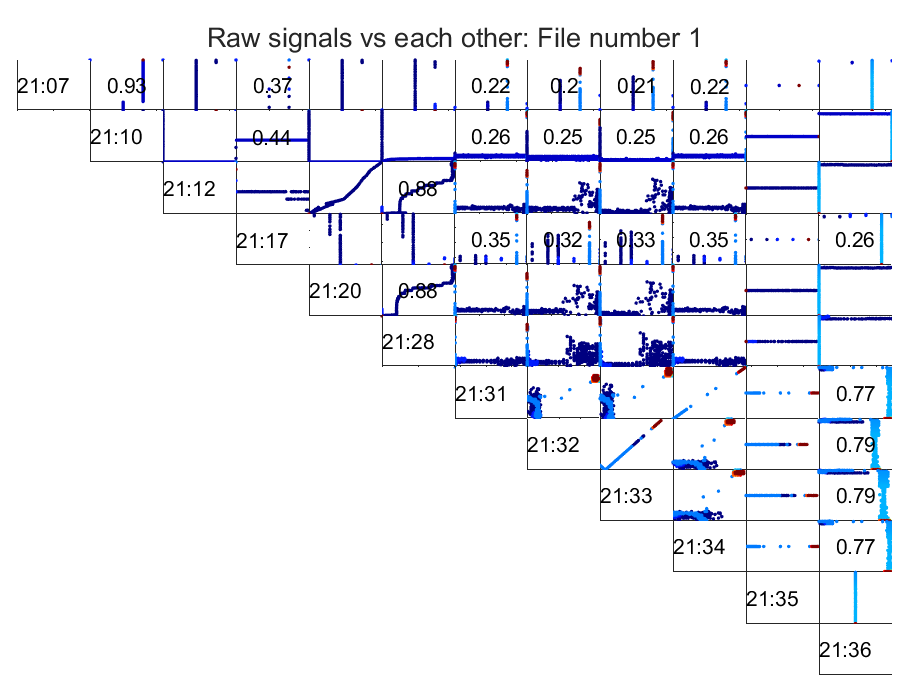
\includegraphics[width=\textwidth, height=\textheight, keepaspectratio]{figures/RawSignalCorrelationsFile1.eps}
    \caption{Plot of each signal vs every other signal with R-square values between 0.2 and 0.9}
    \label{fig:RawSignalCorrelationsFile1}
\end{figure}

\begin{figure}[H]
    \centering
    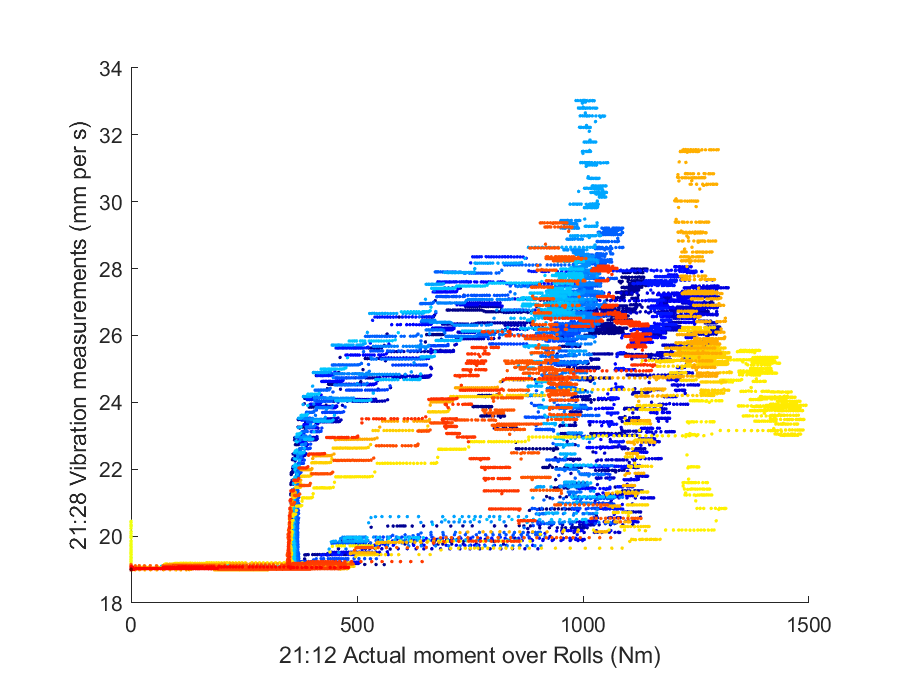
\includegraphics[width=\textwidth, height=\textheight, keepaspectratio]{figures/Signal21_12vSignal21_28.eps}
    \caption{Signal 21.12 v Signal 21 .28}
    \label{fig:Signal21_12vSignal21_28}
\end{figure}

\subsection{Pre-processing}
State detection for this application is performed using Signal 5: 21:20 Actual moment under Rolls. When the machine is not actively processing a tube this value is much less than when it is processing a tube. When no tube is in the system there is no or minimal torque on this sensor and when processing it experiences a much larger moment.
The data is separated into cycles using this signal to isolate the periods where the machine is in the act or processing a part. A threshold of 600 was used as the threshold and a threshold of X samples was also used to filter out short pulses which aren't believed to be full cycles.

Figure \ref{fig:StateDetection} shows the windows that were identified from each file where the 21.20 signal was above the threshold. Two files, B\_30\_03 and B\_04\_04, contained no identified pulses. In total 240 pulses were identified where the 21.20 signal crosses the threshold. Some of these identified pulses were too short and thus believed to be false positives. Any pulse under 500 samples (10 seconds) was removed from the data for the next stage leaving 224 pulses to extract features from.

\begin{figure}[H]
    \centering
    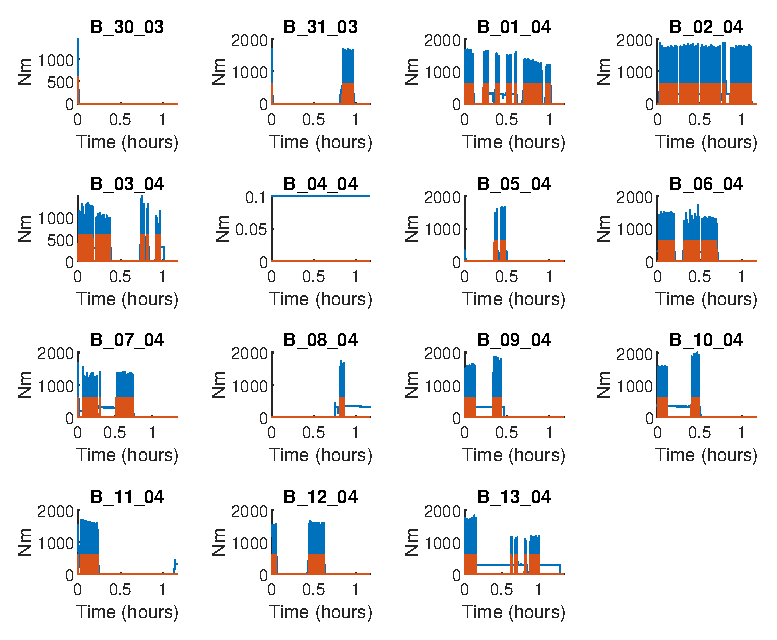
\includegraphics[width=\textwidth, height=\textheight, keepaspectratio]{figures/StateDetectionFig.eps}
    \caption{State detection signal vs 21:20 Actual moment under Rollers}
    \label{fig:StateDetection}
\end{figure}

Figure \ref{fig:StateDetectionFig_B_02_04} shows one of the plots from Figure \ref{fig:StateDetection}, B\_02\_04, in greater detail. This particular file is the one with the highest number of pulses.

\begin{figure}[H]
    \centering
    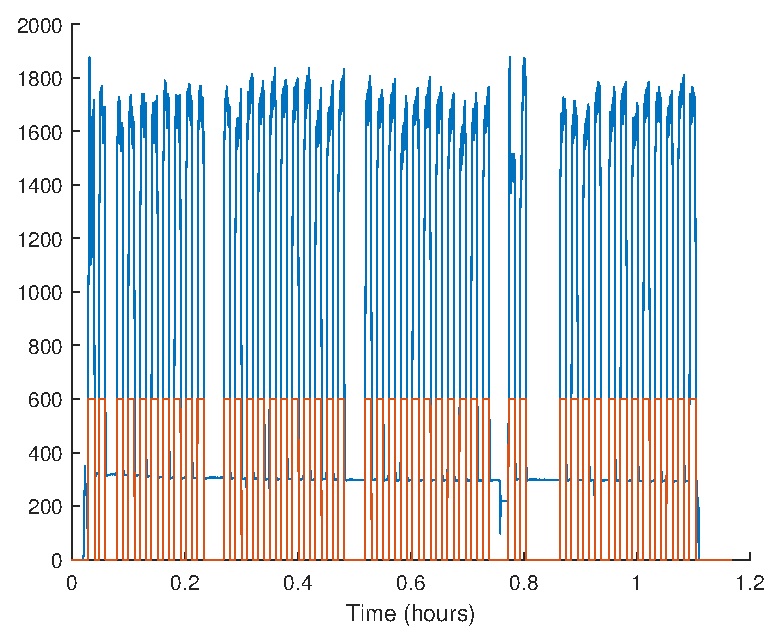
\includegraphics[scale=0.75]{figures/StateDetectionFig_B_02_04.eps}
    \caption{State detection for signal 21:20 performed on file B\_02\_04}
    \label{fig:StateDetectionFig_B_02_04}
\end{figure}

Figure \ref{fig:IdentifiedPulses} shows pulses or cycles for the signal 21:20 in each of the fifteen files. As mentioned earlier B\_30\_03 and B\_04\_04 show no pulses as all. All the pulses are around 40 seconds in duration with similar shapes but varying profiles.
 
\begin{figure}[H]
    \centering
    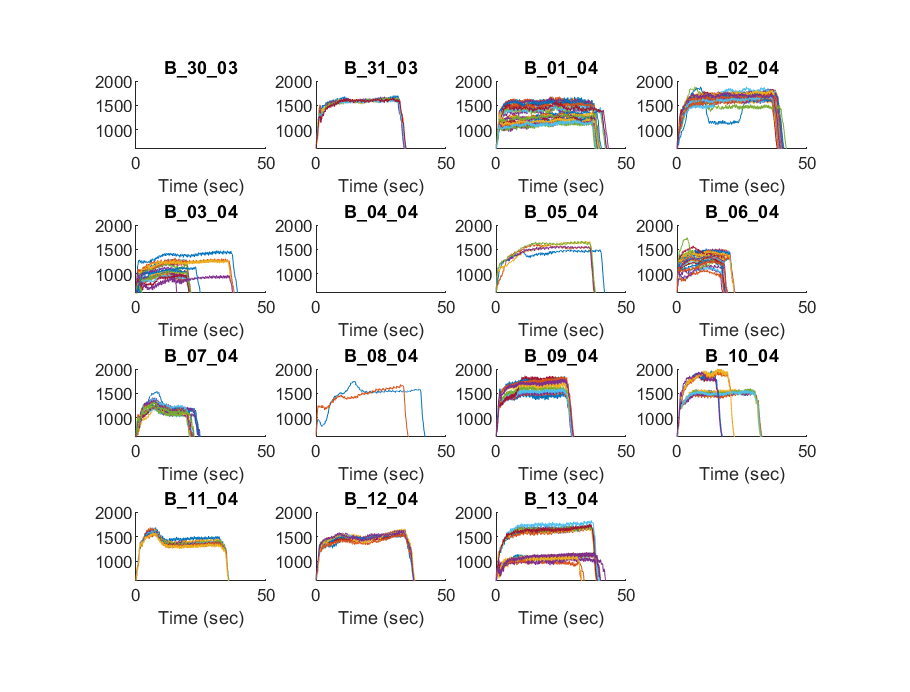
\includegraphics[width=\textwidth, height=\textheight, keepaspectratio]{figures/IdentifiedPulsesFig.eps}
    \caption{Identified pulses in each files for file}
    \label{fig:IdentifiedPulses}
\end{figure}

Figure \ref{fig:SignalPulses} shows the signals for 224 pulses. Each sensor channel is plotted a different tile. 
\begin{figure}[H]
    \centering
    \includegraphics[width=\textwidth, height=\textheight, keepaspectratio]{figures/SignalPulses.eps}
    \caption{Signal pulses for 224 pulses on each of the 12 signal channels}
    \label{fig:SignalPulses}
\end{figure}

Using the identified pulses, we can look at all the other signals during the same periods. Signal 1: 21.07 Angle over Rolls and 2: 21.10 Position over Rolls are fairly constant though contain some small deviations. Signal 7: 21:31 Width position and  8: 21:32 Height position are also fairly constant but contain some information when zoomed in. Signal 21.35 is a fully constant signal and contains nothing but a single value. The label for this signal is set point so it can be assumed that this is a set point that is controlled by the operator and not as sensor on the machine providing feedback. Apart from using this signal for further separating the data into different categories it's likely not that useful for condition monitoring.

Figure \ref{fig:SignalPulse5} shows the state detection, Signal 5: Moment under rolls, signal in more detail. Visually one can see these are a type of pulse single with a small amplitude frequency component. Signal 3: Moment over rolls looks like a very similar type of signal. Channel 6, 9, 10 and 11 contain some interesting information that can be used for characterize the machine state.

%\begin{figure}[H]
%    \centering
%    \includegraphics[scale = 0.75, keepaspectratio]{figures/SignalPulse1.eps}
%    \caption{Signal 1 Pulses 21:07 Angle over Rolls (deg)}
%    \label{fig:SignalPulse1}
%\end{figure}
 
 
%\begin{figure}[H]
%    \centering
%    \includegraphics[scale = 0.75, keepaspectratio]{figures/SignalPulse3.eps}
%    \caption{Signal 3 Pulses 21:12 Actual moment over Rolls (Nm)}
%    \label{fig:SignalPulse3}
%\end{figure}


Figure \ref{fig:SignalPulse5} shows 
\begin{figure}[H]
    \centering
    \includegraphics[scale = 0.75, keepaspectratio]{figures/SignalPulse5.eps}
    \caption{Signal 5 Pulses 21:20 Actual moment under Rolls (Nm)}
    \label{fig:SignalPulse5}
\end{figure}


%\begin{figure}[H]
%    \centering
%    \includegraphics[scale = 0.75, keepaspectratio]{figures/SignalPulse6.eps}
%    \caption{Signal 6 Pulses 6 21:28 Vibration measurements (mm/s)}
%    \label{fig:SignalPulse6}
%\end{figure}

 
%\begin{figure}[H]
%    \centering
%    \includegraphics[scale = 0.75, keepaspectratio, keepaspectratio]{figures/SignalPulse11.eps}
%    \caption{Signal 11 Pulses 21:35 Set point force (kN)}
%    \label{fig:SignalPulse11}
%\end{figure}

\subsection{Feature Selection}
Once the data has been prepossessed and the features calculated then the analysis can begin. Firstly, let us consider a single sensor or channel. Feature values are calculated for each production cycle of this channel. The R-squared value for each pair of features is computed and they are plotted against each other. This is used as a first stage for filtering out irrelevant data. A small, or zero, R-squared value indicates that there is a very weak or no linear relationship between that pair of features. On the other hand an R-squared value of close to 1 indicates that the two features are perfectly or close to perfectly linear. Neither of these feature pairs are of interest as these are not combinations where signals are varying and unlikely to see degradation trends. 

A range of two threshold values are used for this method to select feature pairs. An upper and and a lower R-squared threshold value reveals feature pairs which are somewhat linear or varying in nature. These are the combinations that are of interest to look for condition indicators.

A semi-automated method can be used to narrow down on feature pairs of interest. An algorithm can cycle through the table of R-squared values and the features correlated to a number of others can be isolated. Within that combination one can then remove those signals from the group which are highly correlated with each other.

Not only can one compare pairs of feature within the same signal but one can also look for relationships between the same feature in varying channels or sensors. 

MATLAB's Diagnostic Feature Designer was used calculate the features from the signal pulse data with Table \ref{signalNames} showing the features that were extracted. Throughout the remainder of the report some figures are labeled with a feature number instead of the full text due to readability and space constraints. Use Table \ref{signalNames} to refer to which feature the indexes represents.
\begin{center}
\begin{tabular}{ |c|l| }
 \hline
 1 & Clearance Factor \\
 \hline
 2 & Crest Factor \\
 \hline
 3 & Impulse Factor \\
 \hline
 4 & Kurtosis \\
 \hline
 5 & Mean \\
 \hline
 6 & Peak Value \\
 \hline
 7 & Root Mean Square (RMS) \\ 
 \hline              
 8 & Signal to Noise Ratio (SNR) \\
 \hline
 9 & Signal-to-noise and Distortion Ratio (SINAD) \\
 \hline
 10 & Shape Factor \\
 \hline
 11 & Skewness \\
 \hline
 12 & Standard Deviation \\
 \hline
 13 & Total Harmonic Distortion (THD) \\
 \hline
 14 & Band Power \\
 \hline
 15 & Peak Amplitude 1 \\
 \hline
 16 & Peak Frequency 1 \\
 \hline
\end{tabular}
 \captionof{table}{Feature Names}\label{featureNames}
\end{center}

\subsection{Feature Extraction}

\subsubsection{Feature vs Feature}

%\begin{figure}[H]
%    \centering
%    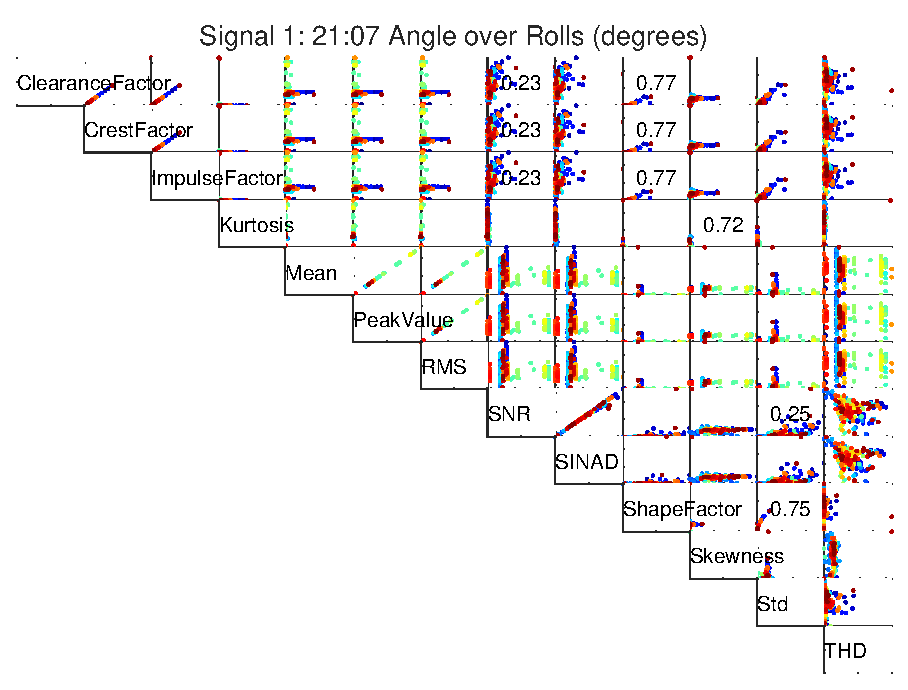
\includegraphics[width=\textwidth, height=\textheight, keepaspectratio]{figures/FeatureVsFeatureSignal1.eps}
%    \caption{Feature Vs Feature for Signal 1 21.07}
%    \label{fig:FeatureVsFeatureSignal1}
%\end{figure}
Figure \ref{fig:FeatureVsFeatureCombinedSignal3} shows an example of plotting all features against one another for signal 1: 21.07 Angle over Rolls. Each number on the diagonal represents a feature starting with the time domain followed by the frequency domain. Only the R-squared values between 0.3 and 0.8 are printed on the relevant plots. It can be noted that features 1, 2 and 3 all have very straight lines for the plots so here we can say that these features (Clearance, Crest and Impulse Factor), are extremely linear and need only include one of these in a model.
The colours used in these plots are used to represent pseudo time. Although since the data is only from 1 hour per day the colour spectrum is not linear however it should be good enough to show a trend over time.
\begin{figure}[H]
    \centering
    \includegraphics[width=\textwidth, height=\textheight, keepaspectratio]{figures/FeatureVsFeatureCombinedSignal3.eps}
    \caption{Feature Vs Feature for Signal 3, Actual moment over Rolls}
    \label{fig:FeatureVsFeatureCombinedSignal3}
\end{figure}

Looking at Feature 1 for this channel, it can be seen that the R-square value is within our range when compared with Feature 10 Kurtosis and Feature 11 Skewness. Figure \ref{fig:Models_Signal3Feature1} shows these three features plotted against one another for all cycles. As expected they are somewhat similar in pattern but not exactly the same.
\begin{figure}[H]
    \centering
    \includegraphics[scale = 0.75, keepaspectratio]{figures/Models_Signal3Feature1.eps}
    \caption{Signal 3 Feature 1}
    \label{fig:Models_Signal3Feature1}
\end{figure}
Likewise in this example is may also be of interest to look at combinations including Features 10 (Figure \ref{fig:Models_Signal3Feature10}), 11 (Figure \ref{fig:Models_Signal3Feature11}) and 14 (Figure \ref{fig:Models_Signal3Feature14}).
\begin{figure}[H]
    \centering
    \includegraphics[scale = 0.75, keepaspectratio]{figures/Models_Signal3Feature10.eps}
    \caption{Signal 3 Feature 10}
    \label{fig:Models_Signal3Feature10}
\end{figure}
 
\begin{figure}[H]
    \centering
    \includegraphics[scale = 0.75, keepaspectratio]{figures/Models_Signal3Feature11.eps}
    \caption{Signal 3 Feature 11}
    \label{fig:Models_Signal3Feature11}
\end{figure}
 
\begin{figure}[H]
    \centering
    \includegraphics[scale = 0.75, keepaspectratio]{figures/Models_Signal3Feature14.eps}
    \caption{Signal 3 Feature 14}
    \label{fig:Models_Signal3Feature14}
\end{figure}


Figure \ref{fig:Models_Signal5Feature1} shows 
\begin{figure}[H]
    \centering
    \includegraphics[width=\textwidth, height=\textheight, keepaspectratio]{figures/Models_Signal5Feature1.eps}
    \caption{Signal 5 Feature 1}
    \label{fig:Models_Signal5Feature1}
\end{figure}



Figure \ref{fig:Models_Signal6Feature1} shows 
\begin{figure}[H]
    \centering
    \includegraphics[width=\textwidth, height=\textheight, keepaspectratio]{figures/Models_Signal6Feature1.eps}
    \caption{Signal 6 Feature 1}
    \label{fig:Models_Signal6Feature1}
\end{figure}


Figure \ref{fig:Models_Signal9Feature3} shows 
\begin{figure}[H]
    \centering
    \includegraphics[width=\textwidth, height=\textheight, keepaspectratio]{figures/Models_Signal9Feature3.eps}
    \caption{Signal 9 Feature 3}
    \label{fig:Models_Signal9Feature3}
\end{figure}
Figure \ref{fig:Models_Signal9Feature4} shows 
\begin{figure}[H]
    \centering
    \includegraphics[width=\textwidth, height=\textheight, keepaspectratio]{figures/Models_Signal9Feature4.eps}
    \caption{Signal 9 Feature 4}
    \label{fig:Models_Signal9Feature4}
\end{figure}
Figure \ref{fig:Models_Signal9Feature11} shows 
\begin{figure}[H]
    \centering
    \includegraphics[width=\textwidth, height=\textheight, keepaspectratio]{figures/Models_Signal9Feature11.eps}
    \caption{Signal 9 Feature 11}
    \label{fig:Models_Signal9Feature11}
\end{figure}

\subsubsection{Signal vs Signal}
Figure \ref{fig:SignalVsSignalFeatureTime1} shows 
\begin{figure}[H]
    \centering
    \includegraphics[width=\textwidth, height=\textheight, keepaspectratio]{figures/SignalVsSignalFeatureTime1.eps}
    \caption{Signal Vs Signal for Time Feature 1}
    \label{fig:SignalVsSignalFeatureTime1}
\end{figure}


Figure \ref{fig:Models_Feature5Signal1} shows 
\begin{figure}[H]
    \centering
    \includegraphics[width=\textwidth, height=\textheight, keepaspectratio]{figures/Models_Feature5Signal1.eps}
    \caption{Feature 5 Signal 1}
    \label{fig:Models_Feature5Signal1}
\end{figure}


Figure \ref{fig:Models_Feature14Signal1} shows 
\begin{figure}[H]
    \centering
    \includegraphics[width=\textwidth, height=\textheight, keepaspectratio]{figures/Models_Feature14Signal1.eps}
    \caption{Feature 14 Signal 1}
    \label{fig:Models_Feature14Signal1}
\end{figure}

Figure \ref{fig:Models_Feature16Signal3} shows 
\begin{figure}[H]
    \centering
    \includegraphics[width=\textwidth, height=\textheight, keepaspectratio]{figures/Models_Feature16Signal3.eps}
    \caption{Feature 16 Signal 3}
    \label{fig:Models_Feature16Signal3}
\end{figure}

Figure \ref{fig:Models_Feature16Signal3_Linear1} shows the peak frequency of the Actual Moment over Rolls vs Actual moment under Rolls. It can be noted that a majority of the data points follow the a linear model very well. However, a subset of the available data appear to form another linear relationship with a similar gradient but slightly lower intercept.
\begin{figure}[H]
    \centering
    \includegraphics[width=\textwidth, height=\textheight, keepaspectratio]{figures/Models_Feature16Signal3_Linear1.eps}
    \caption{Feature 16 Signal 3 Linear 1}
    \label{fig:Models_Feature16Signal3_Linear1}
\end{figure}

\subsection{Linear Models}

\subsection{Multivariate Models}

\clearpage 

\section{Discussion}
%Discuss results and put in context/comparison with references at the beginning. 
This study aimed to give suggestions as to what signals and/or signal features are of value for future condition monitoring studies and which ones are not.

The work performed in this study has been limited to an analysis of the available data. Future work could include the application of machine learning techniques to the signals highlighted in this project. In particular unsupervised learning approaches such as K nearest neighbors or K-means clustering approach.

The data supplied for the project is from a two week period which probably does not give a good insight into the life cycle of the machine. Perhaps a better selection of data would include a snippet of data every 1-2 weeks and thus one could get a better view of how the machine degrades over a year.

The straightening machine in this study produces products of of different diameters. At least one of the signals can be used to indicate this diameter. This could be used to classify the data further into different tube widths. A suggestion for future studies is to perform an additional prepossessing step to separate data into periods where the machine is producing tubes with certain diameters. Some of the clustering suggestions or relationships given in this study could just be identifying when the machine is producing a tube of a certain width. Separating data and focusing on only one tube width would removed any chance of this. A method like this would have been challenging since only 224 pulses were identified to begin with and thus a further reduction might result in not enough data to make meaningful observations.

One conclusion could be that "for future condition monitoring work we need to only focus on this data (might only be 10\%)".\\
Another conclusion could be that we need to go forward to doing this and that.\\
Conclusion could be what we say to the company or what we need.\\
Would temperature of something be good to monitor?\\
Worth doing an analysis based on different sizes
Ideally we would have data over the lifespan of a machine. The data we have right know, we don't know whether is is normal operating data. It could be right at the beginning of the lifecycle or could be just at the end of the machines lifecycle. A system that has been operating for a long period of time will undergo changes due to the natural wear of the system.
One conclusion might be just to discard all the signals with constant values.
These types of analysis can be expanded exponentially but one can only look at so much before moving on. It is also beneficial to, at least begin with, simple things like two variable linear regression.

Since 2017 it is mandatory that all technical reports, theses, and similar publications, discuss Environmental Impact and Sustainability of the project. To find a starting point it is suggested to use “the United Nations’ 2030 Agenda for Sustainable Development” and its 17 Sustainable Development Goals (www.un.org/sustainabledevelopment/development-agenda). Under each goal there are some goal targets listed. Identify one or more goals relevant for your thesis, and comment using relevant goal targets.
It should also be noted that the result and the methods used in this thesis are in good agreement with target 9.5 of the 2030 Agenda for sustainable development [52].
\clearpage

\section{Conclusion}
A study of the available data on a steel tube straightening machine was conducted with regards to using the existing infrastructure for condition monitoring.
\begin{itemize}
\item Correlation was performed on the raw signal data to identify relationships between the sensor channels.
\item The data was prepossessed using an amplitude threshold for the state detection and then a time threshold to eliminate false cycles.
\item Time and frequency domain features were extracted from the cycles.
\item For every sensor channel, each feature was plotted against every other feature and the R-squared correlation coefficient was calculated.
\item An upper and lower threshold, was used to selected a combination of features that are somewhat correlated but not well perfectly correlated.

\end{itemize}


\newpage

\section{References} 
\printbibliography[heading=none] 
\clearpage  
\section{Appendix A - Matlab Code}
\UseRawInputEncoding
\lstinputlisting[frame=single, numbers=left, style=Matlab-editor]{"./MATLAB Software/LoadRawData.m"}
\lstinputlisting[frame=single, numbers=left, style=Matlab-editor]{"./MATLAB Software/LoadFeatures.m"}
%\lstinputlisting[frame=single, numbers=left, style=Matlab-editor]{"./MATLAB Software/PreProcessData.mlx"}
\end{document}